% Render: latex gears.tex && dvisvgm --no-fonts --bbox=papersize gears.dvi -o gears.svg
% What an agent assembles. The chains are the `deps` of each gear's #[toolkit::gear]
% declaration in constructorfabric/gears-rust (src/nextgear/fabric_gears.py).
\documentclass[tikz,border=12pt]{standalone}
\pagecolor{white}
\usetikzlibrary{arrows.meta,positioning}

\begin{document}
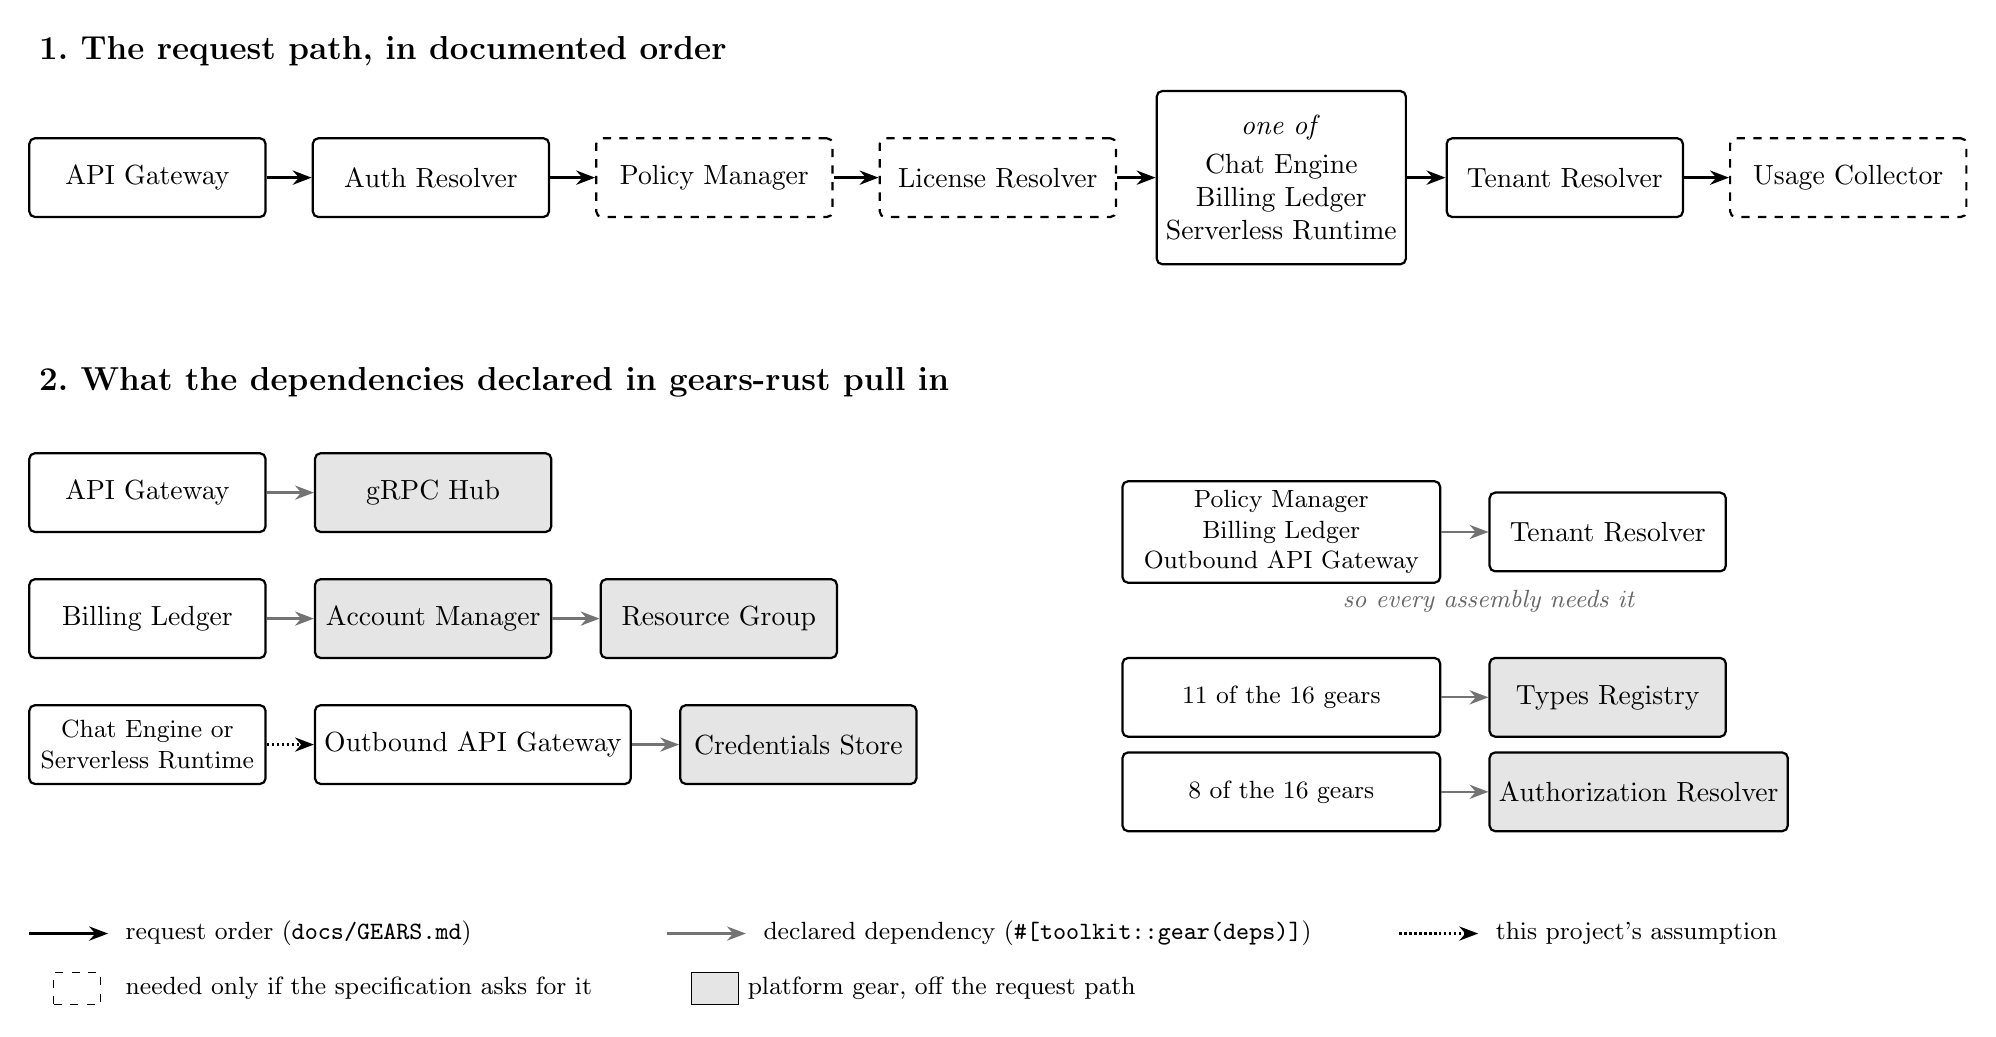
\begin{tikzpicture}[
  >={Stealth[length=2.4mm]},
  gear/.style={draw, thick, rounded corners=2pt, minimum width=30mm, minimum height=10mm, align=center, fill=white},
  optional/.style={gear, dashed},
  platform/.style={gear, fill=black!10},
  order/.style={->, very thick},
  dep/.style={->, thick, black!55},
  assumed/.style={->, thick, densely dotted},
  heading/.style={font=\large\bfseries, anchor=west},
  note/.style={font=\small\itshape, text=black!60, anchor=north west},
  node distance=6mm,
]

% 1. The request path, in the order docs/GEARS.md gives.
\node[heading] at (-1.5, 1.6) {1.\ The request path, in documented order};
\node[gear]     (api)     at (0, 0)    {API Gateway};
\node[gear]     (authn)   at (3.6, 0)  {Auth Resolver};
\node[optional] (policy)  at (7.2, 0)  {Policy Manager};
\node[optional] (license) at (10.8, 0) {License Resolver};
\node[gear, minimum height=22mm] (exec) at (14.4, 0) {\textit{one of}\\[2pt] Chat Engine\\ Billing Ledger\\ Serverless Runtime};
\node[gear]     (tenant)  at (18, 0)   {Tenant Resolver};
\node[optional] (usage)   at (21.6, 0) {Usage Collector};
\foreach \a/\b in {api/authn, authn/policy, policy/license, license/exec, exec/tenant, tenant/usage}
  \draw[order] (\a) -- (\b);

% 2. What the declared dependencies pull in.
\node[heading] at (-1.5, -2.6) {2.\ What the dependencies declared in gears-rust pull in};

\node[gear]     (c1a) at (0, -4)    {API Gateway};
\node[platform, right=of c1a] (c1b) {gRPC Hub};
\draw[dep] (c1a) -- (c1b);

\node[gear]     (c2a) at (0, -5.6)  {Billing Ledger};
\node[platform, right=of c2a] (c2b) {Account Manager};
\node[platform, right=of c2b] (c2c) {Resource Group};
\draw[dep] (c2a) -- (c2b);
\draw[dep] (c2b) -- (c2c);

\node[gear, font=\small] (c3a) at (0, -7.2) {Chat Engine or\\ Serverless Runtime};
\node[gear, right=of c3a] (c3b) {Outbound API Gateway};
\node[platform, right=of c3b] (c3c) {Credentials Store};
\draw[assumed] (c3a) -- (c3b);
\draw[dep] (c3b) -- (c3c);

\node[gear, text width=38mm, font=\small] (c4a) at (14.4, -4.5)
  {Policy Manager\\ Billing Ledger\\ Outbound API Gateway};
\node[gear, right=of c4a] (c4b) {Tenant Resolver};
\node[note, below=1mm of c4b.south west] {so every assembly needs it};
\draw[dep] (c4a) -- (c4b);

\node[gear, text width=38mm, font=\small] (c5a) at (14.4, -6.6) {11 of the 16 gears};
\node[platform, right=of c5a] (c5b) {Types Registry};
\draw[dep] (c5a) -- (c5b);
\node[gear, text width=38mm, font=\small] (c6a) at (14.4, -7.8) {8 of the 16 gears};
\node[platform, right=of c6a] (c6b) {Authorization Resolver};
\draw[dep] (c6a) -- (c6b);

% Legend.
\begin{scope}[shift={(-1.5, -9.6)}, every node/.style={font=\small, anchor=west}]
  \draw[order] (0, 0) -- (1, 0);         \node at (1.1, 0) {request order (\texttt{docs/GEARS.md})};
  \draw[dep] (8.1, 0) -- (9.1, 0);       \node at (9.2, 0) {declared dependency (\texttt{\#[toolkit::gear(deps)]})};
  \draw[assumed] (17.4, 0) -- (18.4, 0); \node at (18.5, 0) {this project's assumption};
  \node[draw, dashed, minimum width=6mm, minimum height=4mm] at (0.3, -0.7) {};
  \node at (1.1, -0.7) {needed only if the specification asks for it};
  \node[draw, fill=black!10, minimum width=6mm, minimum height=4mm] at (8.4, -0.7) {};
  \node at (9.0, -0.7) {platform gear, off the request path};
\end{scope}
\end{tikzpicture}
\end{document}
